\subsection{Operation Model for oeCreateSystemAndEnvironment}

\label{OM-oeCreateSystemAndEnvironment}


The \msrcode{oeCreateSystemAndEnvironment} operation has the following properties:

	\begin{operationmodel}
	\addheading{Operation}
	\adddoublerow{oeCreateSystemAndEnvironment}{sent to request the initialization of the system's class instances and the environment actors instances.}

	\addrowheading{Parameters}
	\addnumbereddoublerow{}{AqtyComCompanies: ptInteger}{the quantity of communication companies to create in the environment} 

	\addrowheading{Return type}
	\addsinglerow{ptBoolean}

	\addrowheading{Pre-Condition (protocol)}
	\addnumberedsinglerow{PreP}{ none}
		
	\addrowheading{Pre-Condition (functional)}
	\addnumberedsinglerow{PreF}{ none }

	\addrowheading{Post-Condition (functional)}
	\addnumberedsinglerow{PostF}{ the ctState instance is initialized with the integer 1 for the crisis and alert counters used for their identifications, a value for the clock corresponding to a default inital time (i.e. January 1st, 1970) the crisis reminder period is set to 300 seconds, the maximum crisis reminder period is fixed to 1200 seconds (i.e. 20 minutes), an initial value for the automatic reminder period equal to the current date and time and the system is considered in a started state.
	
	{\bf Those predicates must be satisfied first since all the other depend on the existence of a ctState instance !}}
	\addnumberedsinglerow{PostF}{the \msrcode{actMsrCreator} actor instance is initiated (remember that since the \msrcode{oeCreateSystemAndEnvironment} is a special event it role is to make consistent the post state thus creating the actor and its interfaces is required even though the sending of this message logically would need the actor and its interfaces to already exist ...).}
	\addnumberedsinglerow{PostF}{the environment for communication company actors, in the post state, is made of \msrcode{AqtyComCompanies} instances allowing for receiving and sending messages to humans.}
	\addnumberedsinglerow{PostF}{the environment for administrator actors, in the post state, is made of one instance.}
	\addnumberedsinglerow{PostF}{the environment for activator actors, in the post state, is made of one instance allowing for automatic message sending based on current system's and environment state'.}
	\addnumberedsinglerow{PostF}{the set of ctAdministrator instances at post is made of one instance initialized with 'icrashadmin' (resp. '7WXC1359') for login (resp. password) values.}
	\addnumberedsinglerow{PostF}{the association between ctAdministrator and actAdministrator is made of one couple made of the conjointly specified instances.}

	\addrowheading{Post-Condition (protocol)}
	\addnumberedsinglerow{PostP}{ none is given since the only protocol variable to be modified in the post state is the one initialized with the ctState instance (i.e. vpStarted).}
	\end{operationmodel}



	
	
	
	





Figure \ref{fig:lu.uni.lassy.icrash.spec.messir.reference-OM-scopeView-operation-scope-outactMsrCreator-oeCreateSystemAndEnvironment}
shows all the concept model elements in the scope of the oeCreateSystemAndEnvironment operation

\begin{figure}[htbp]
\begin{center}

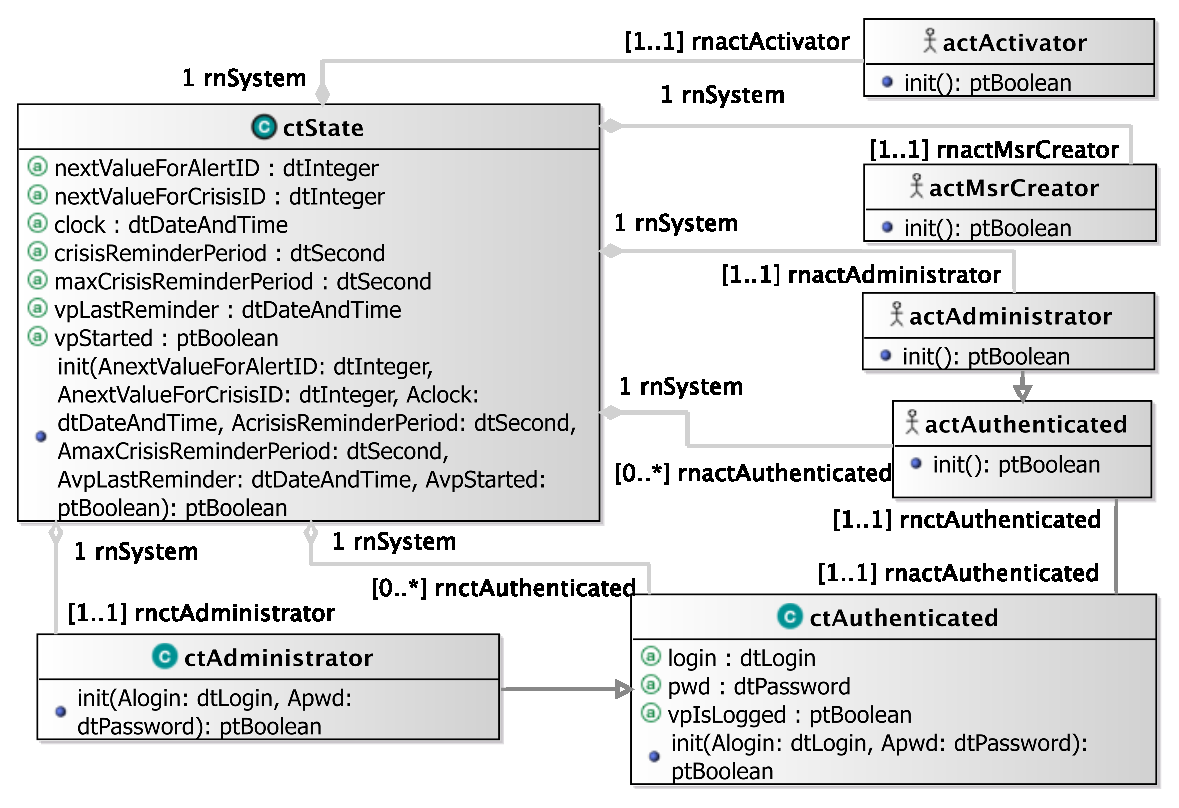
\includegraphics[
angle=0
,width=1.0\textwidth
]{./images-report-gen/operation-model/operation-scope-outactMsrCreator-oeCreateSystemAndEnvironment.eps}
\end{center}
\caption[lu.uni.lassy.icrash.spec.messir.reference Operation Scope: operation-scope-outactMsrCreator-oeCreateSystemAndEnvironment]{oeCreateSystemAndEnvironment operation scope
}
\label{fig:lu.uni.lassy.icrash.spec.messir.reference-OM-scopeView-operation-scope-outactMsrCreator-oeCreateSystemAndEnvironment}
\end{figure}
\vspace{0.5cm}

